% !TEX root = Projektdokumentation.tex
\section{Anhang}

\subsection{Zeitnachweis}
\label{app:Zeitnachweis}
\begin{table}[htbp]
\centering
\begin{tabular}{|p{9cm}|r|}
\hline
\textbf{Tätigkeit} & \textbf{Stunden} \\
\hline
Ist-Analyse und Anforderungsklärung & 8 \\
\hline
Soll-Konzept und Variantenvergleich & 10 \\
\hline
Entwurf von Datenmodell und Rollenmodell & 8 \\
\hline
Entwurf der Weboberfläche und Navigationsstruktur & 4 \\
\hline
Implementierung Stammdatenverwaltung & 10 \\
\hline
Implementierung Benutzer- und Rechteverwaltung & 8 \\
\hline
Implementierung Login-Schutz und Audit-Log & 10 \\
\hline
Tests, Fehlerkorrekturen und Abnahmevorbereitung & 10 \\
\hline
Kundendokumentation und Projektdokumentation & 12 \\
\hline
\textbf{Summe} & \textbf{80} \\
\hline
\end{tabular}
\caption{Zeitnachweis}
\end{table}
\clearpage

\subsection{Wirtschaftlichkeit}
\label{app:Wirtschaftlichkeit}
\begin{table}[htbp]
\centering
\begin{tabular}{|p{7.0cm}|r|r|r|}
\hline
\textbf{Position} & \textbf{Stunden} & \textbf{Satz} & \textbf{Kosten} \\
\hline
Projektdurchführung & 80 & \eur{65} & \eur{5200} \\
\hline
Fachliche Begleitung und Abnahme & 6 & \eur{85} & \eur{510} \\
\hline
Softwarelizenzen & - & - & \eur{0} \\
\hline
\textbf{Gesamt} & & & \textbf{\eur{5710}} \\
\hline
\end{tabular}
\caption{Detailrechnung der Projektkosten}
\end{table}
\clearpage

\subsection{Variantenvergleich}
\label{app:Variantenvergleich}
\begin{table}[htbp]
\centering
\begin{tabular}{|p{4.6cm}|r|r|r|}
\hline
\textbf{Kriterium} & \textbf{Gewicht} & \textbf{Standardlösung} & \textbf{Eigenentwicklung} \\
\hline
Passgenauigkeit & 5 & 3 & 5 \\
\hline
Mandantentrennung und Rechteabbildung & 5 & 3 & 5 \\
\hline
Nachvollziehbarkeit und Auditierung & 4 & 3 & 5 \\
\hline
Einführungsaufwand & 3 & 3 & 4 \\
\hline
Wartbarkeit im Betrieb & 3 & 3 & 4 \\
\hline
\textbf{Gewichteter Nutzwert} & & \textbf{51} & \textbf{80} \\
\hline
\end{tabular}
\caption{Gewichteter Variantenvergleich}
\end{table}
\clearpage

\subsection{Use Case-Diagramm}
\label{app:UseCase}
\begin{figure}[htb]
\centering
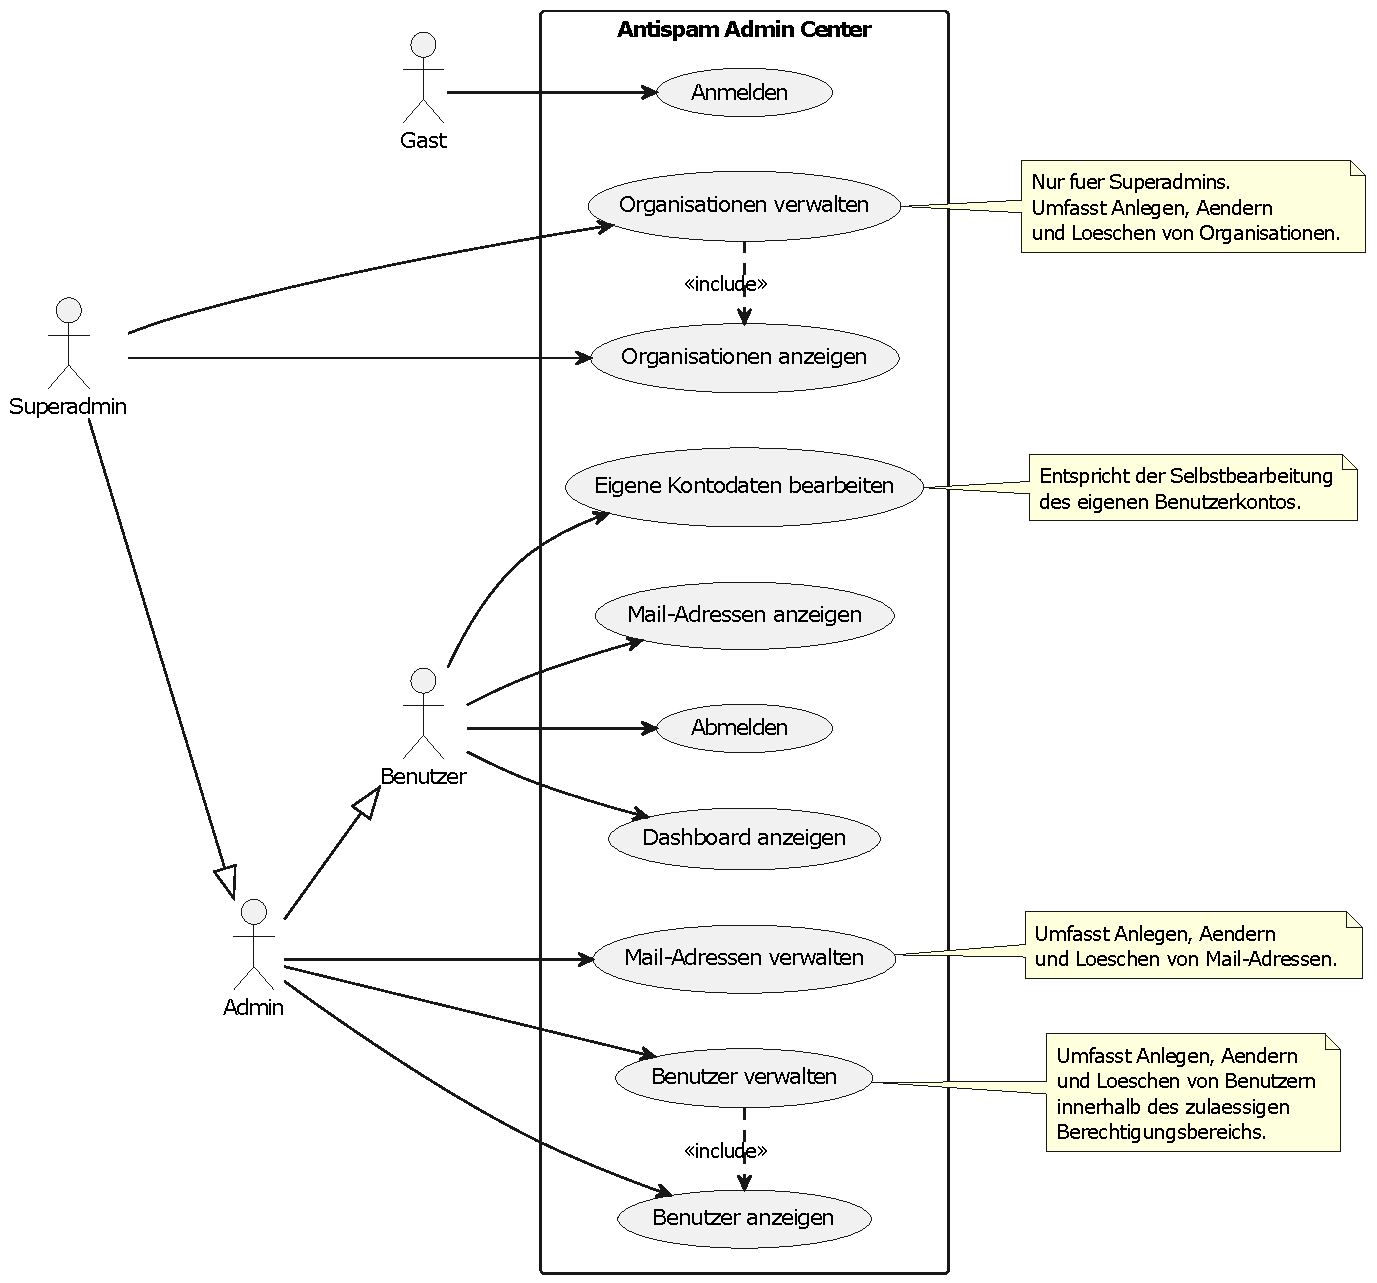
\includegraphics[width=0.9\textwidth]{PlantUML/UseCaseDiagramm.pdf}
\caption{Use Case-Diagramm}
\end{figure}
\clearpage

\subsection{Datenbankmodell}
\label{app:Datenbankmodell}
\begin{figure}[htb]
\centering
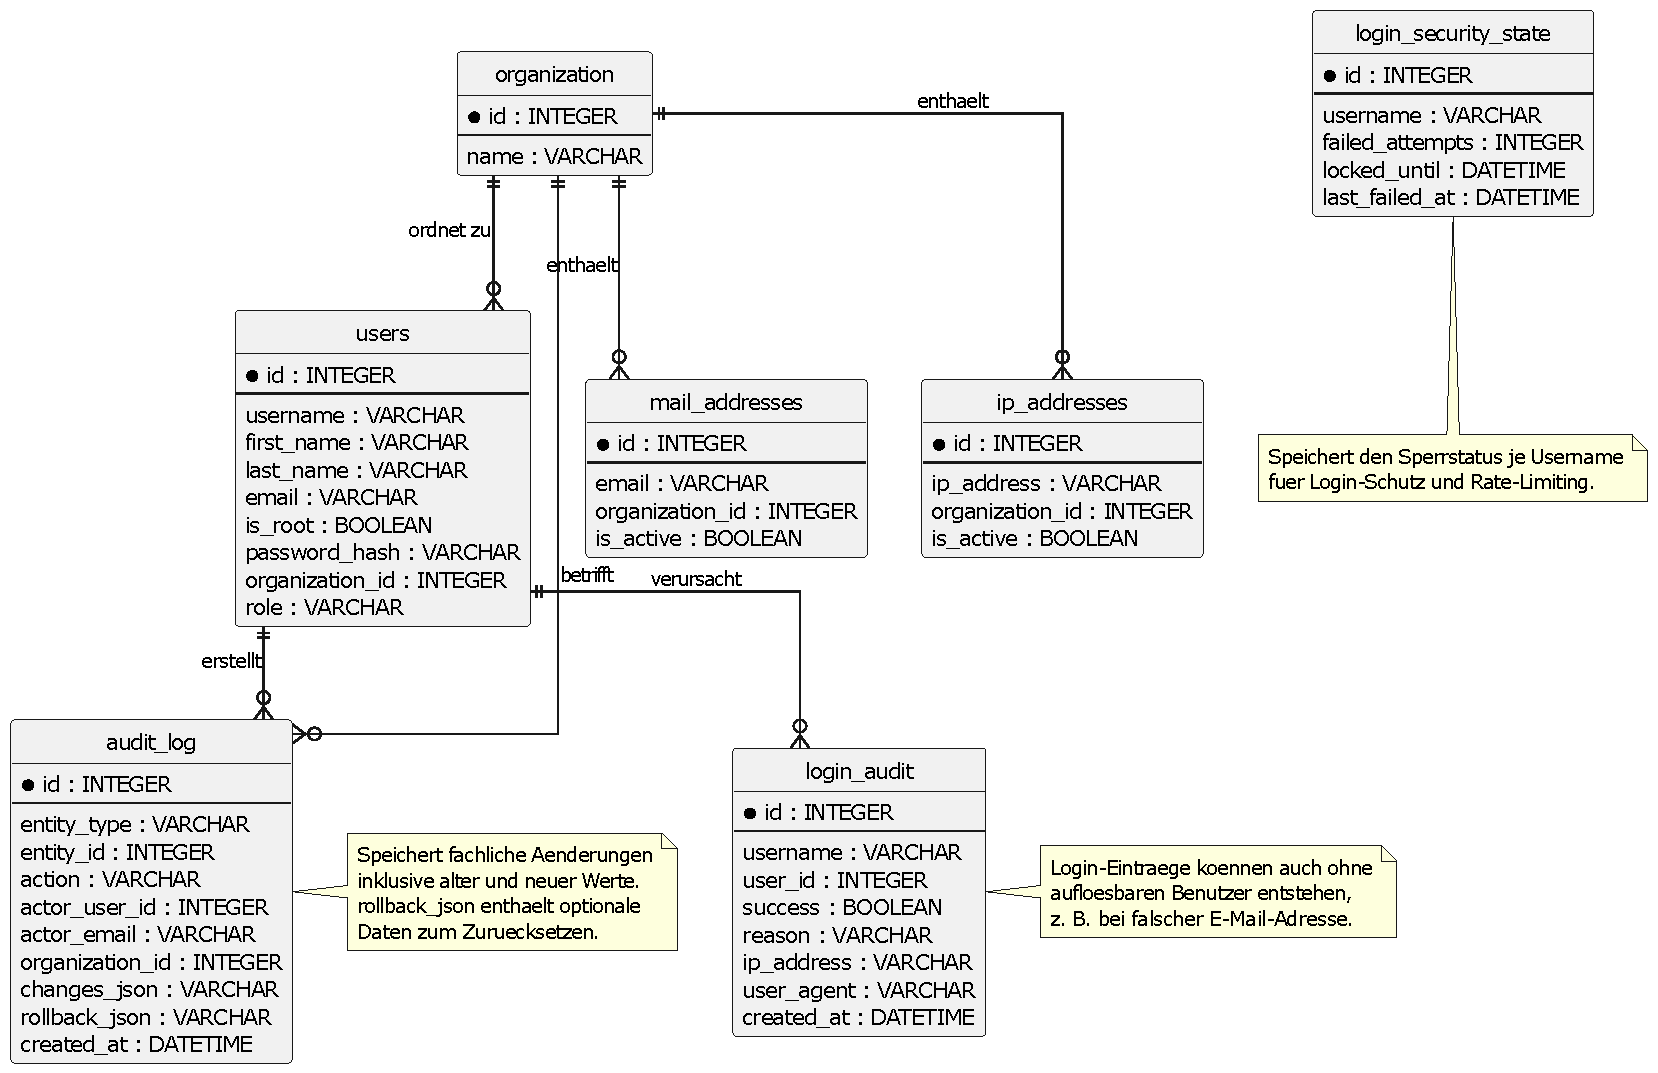
\includegraphics[width=0.95\textwidth]{PlantUML/database.pdf}
\caption{Datenbankmodell}
\end{figure}
\clearpage

\subsection{Klassendiagramm}
\label{app:Klassendiagramm}
\begin{figure}[htb]
\centering
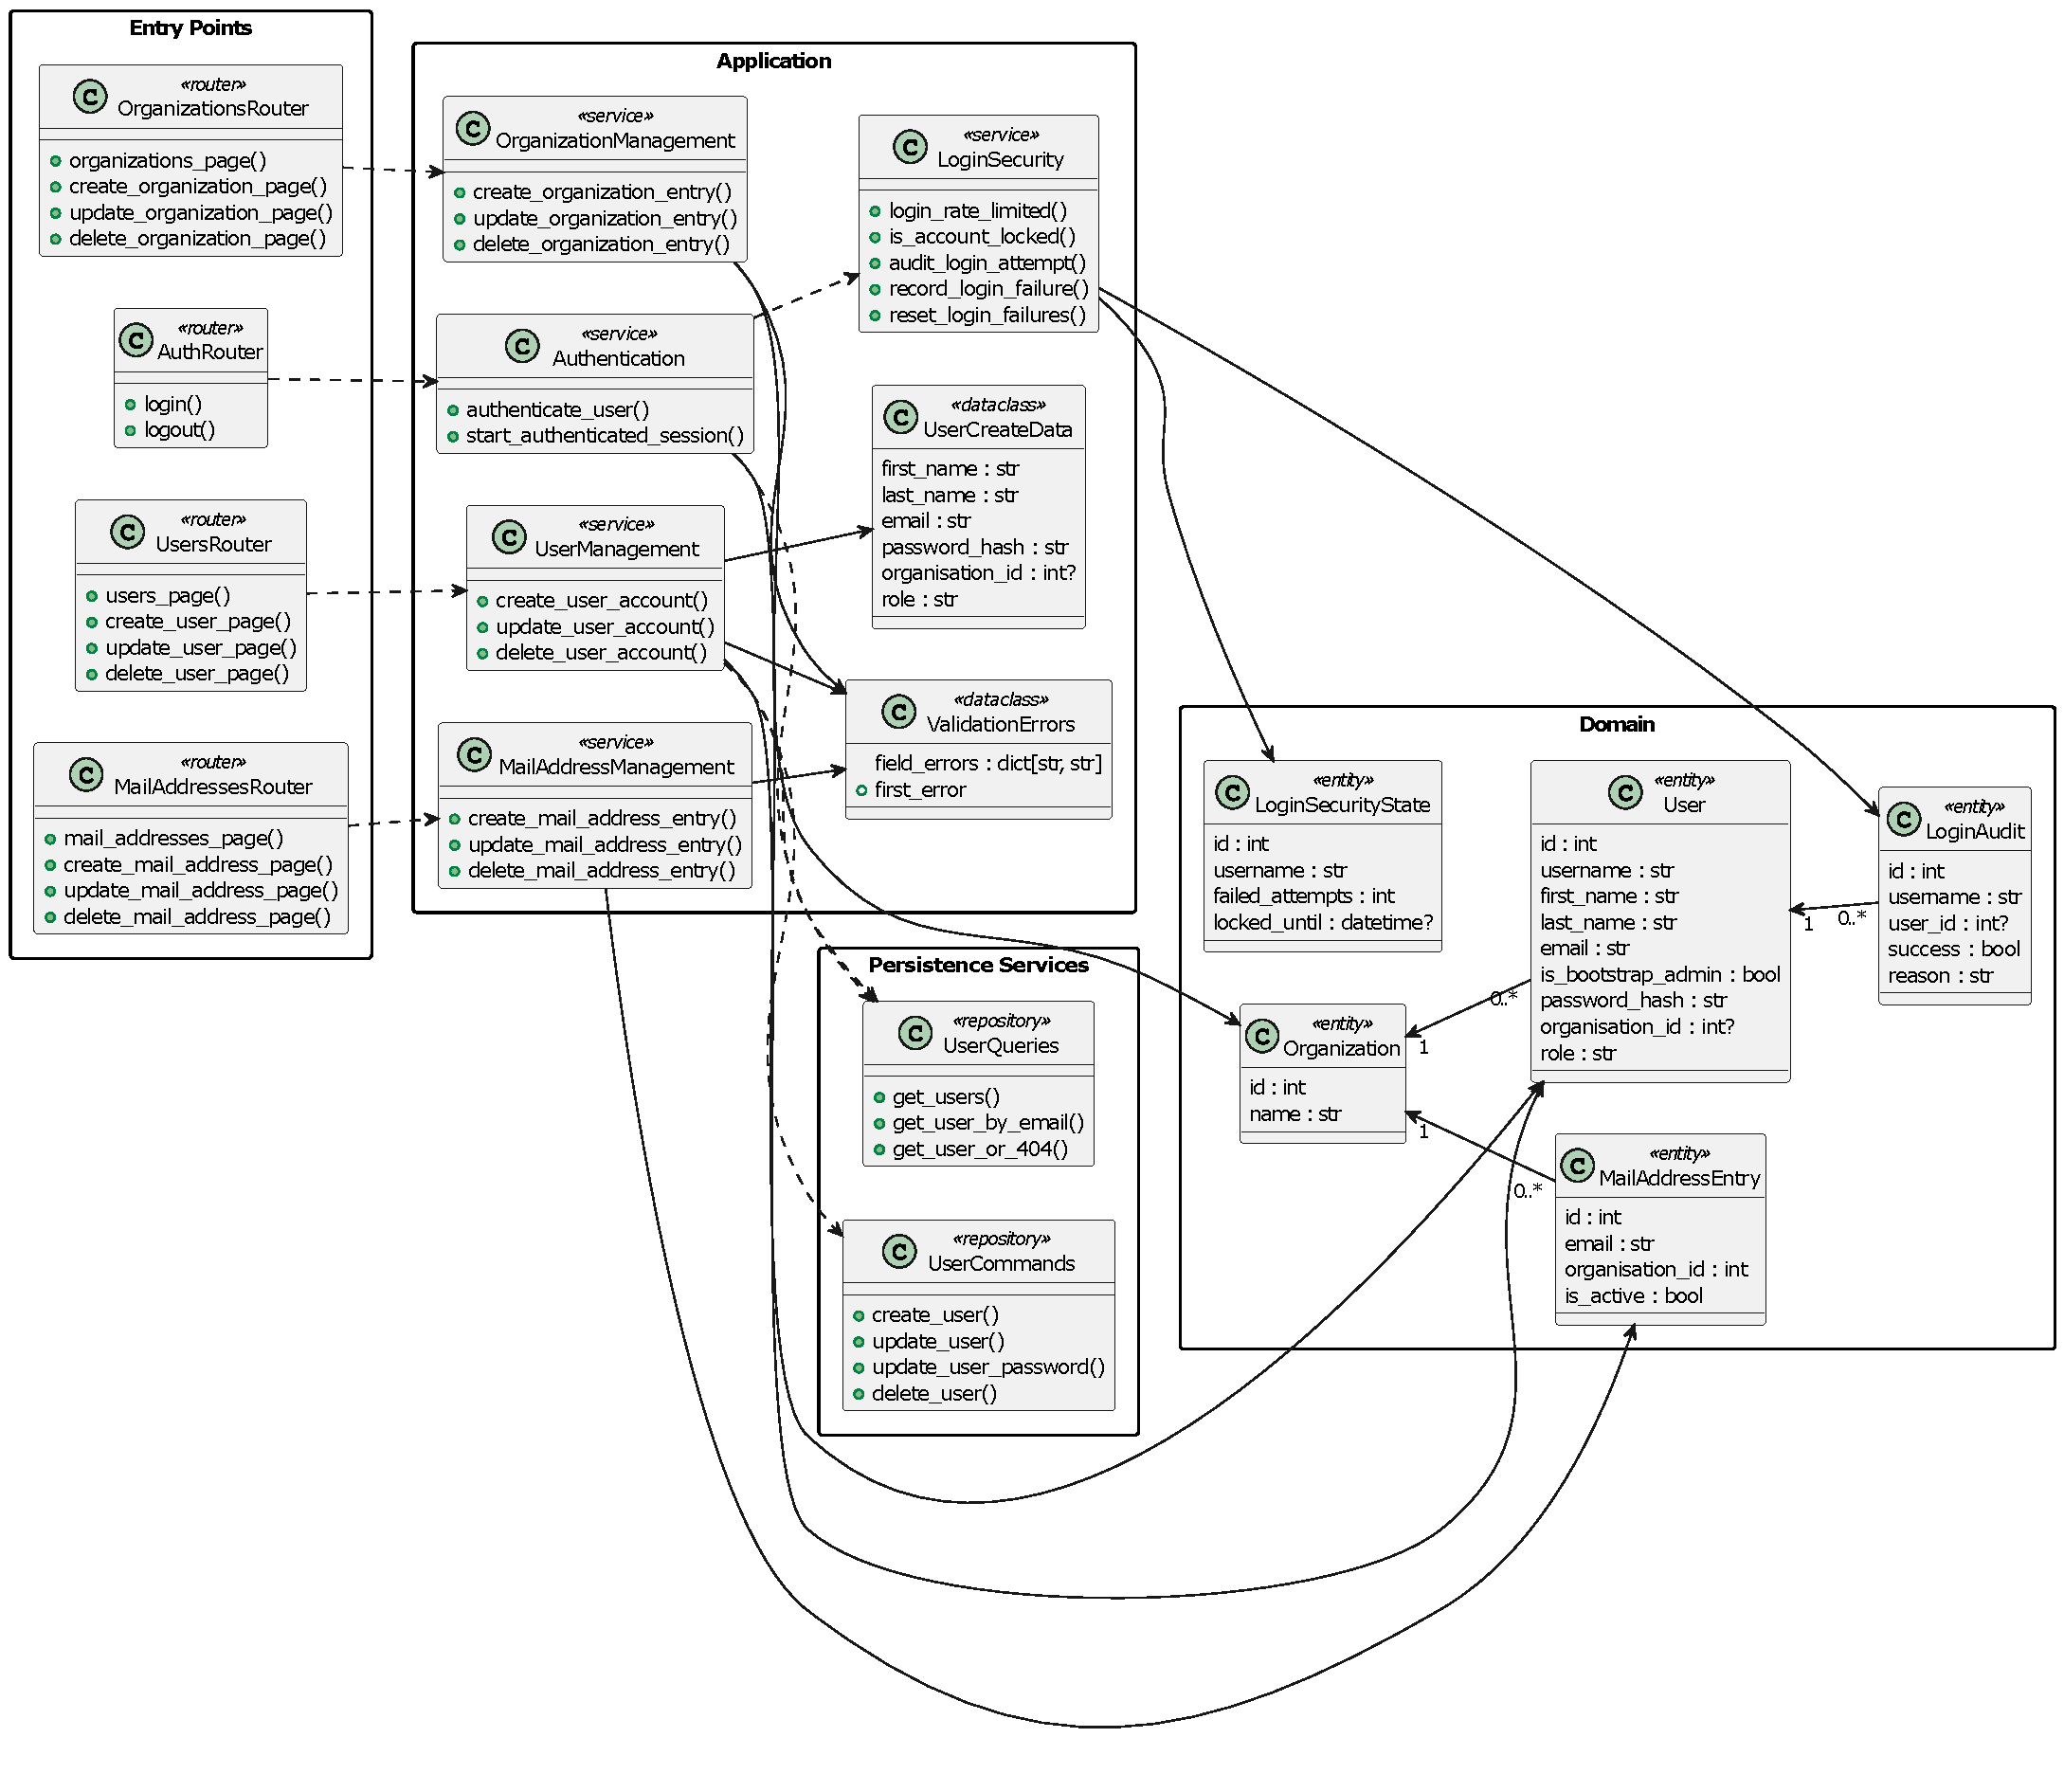
\includegraphics[width=0.95\textwidth]{PlantUML/Klassendiagramm.pdf}
\caption{Klassendiagramm}
\end{figure}
\clearpage

\subsection{Komponentendiagramm}
\label{app:Komponentendiagramm}
\begin{figure}[htb]
\centering
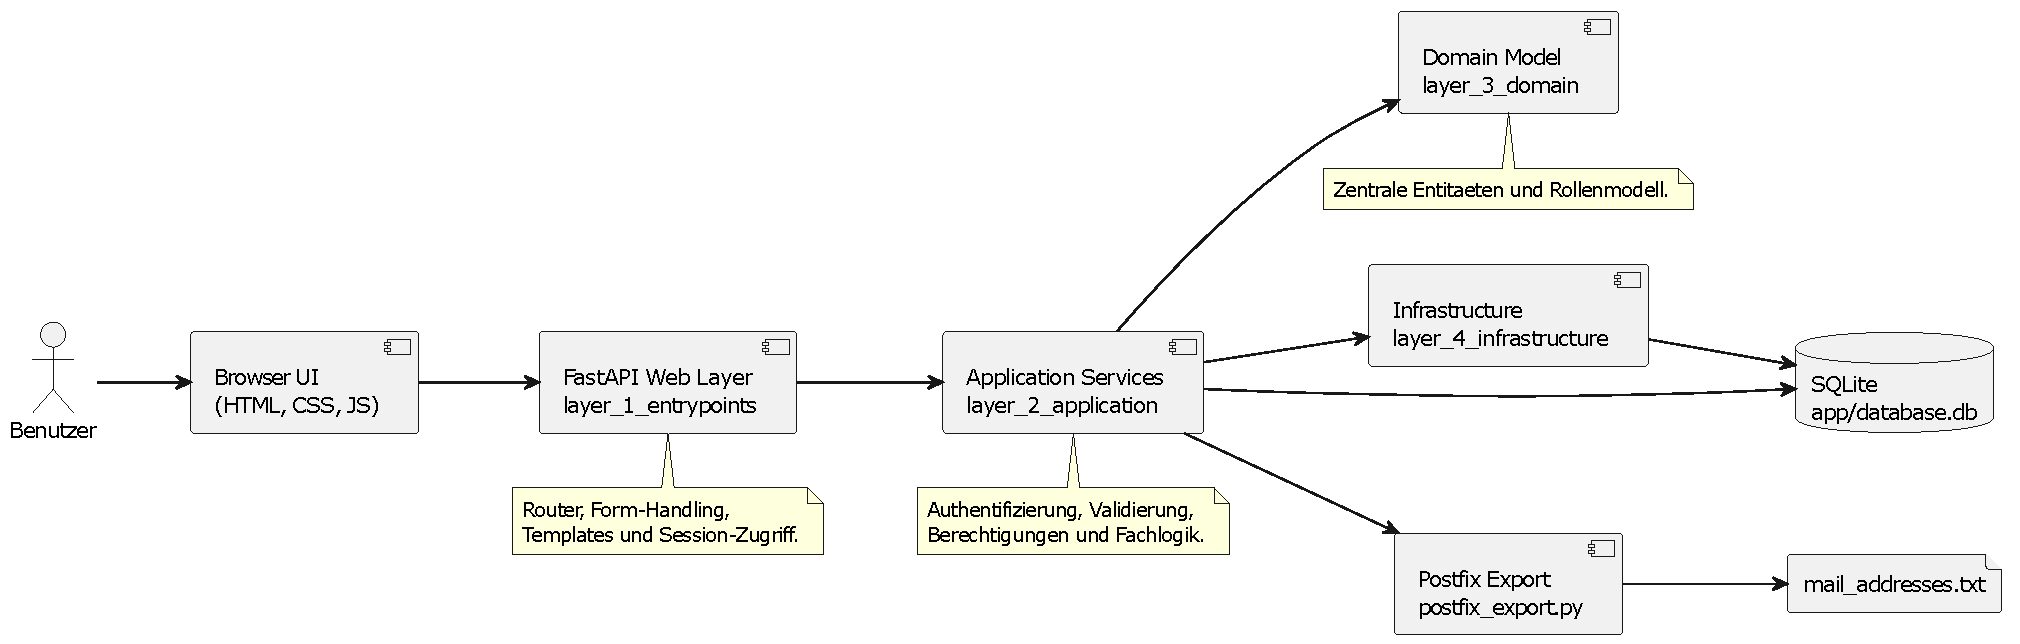
\includegraphics[width=0.95\textwidth]{PlantUML/Komponentendiagramm.pdf}
\caption{Komponentendiagramm}
\end{figure}
\clearpage

\subsection{Sequenzdiagramm Login}
\label{app:SequenzdiagrammLogin}
\begin{figure}[htb]
\centering
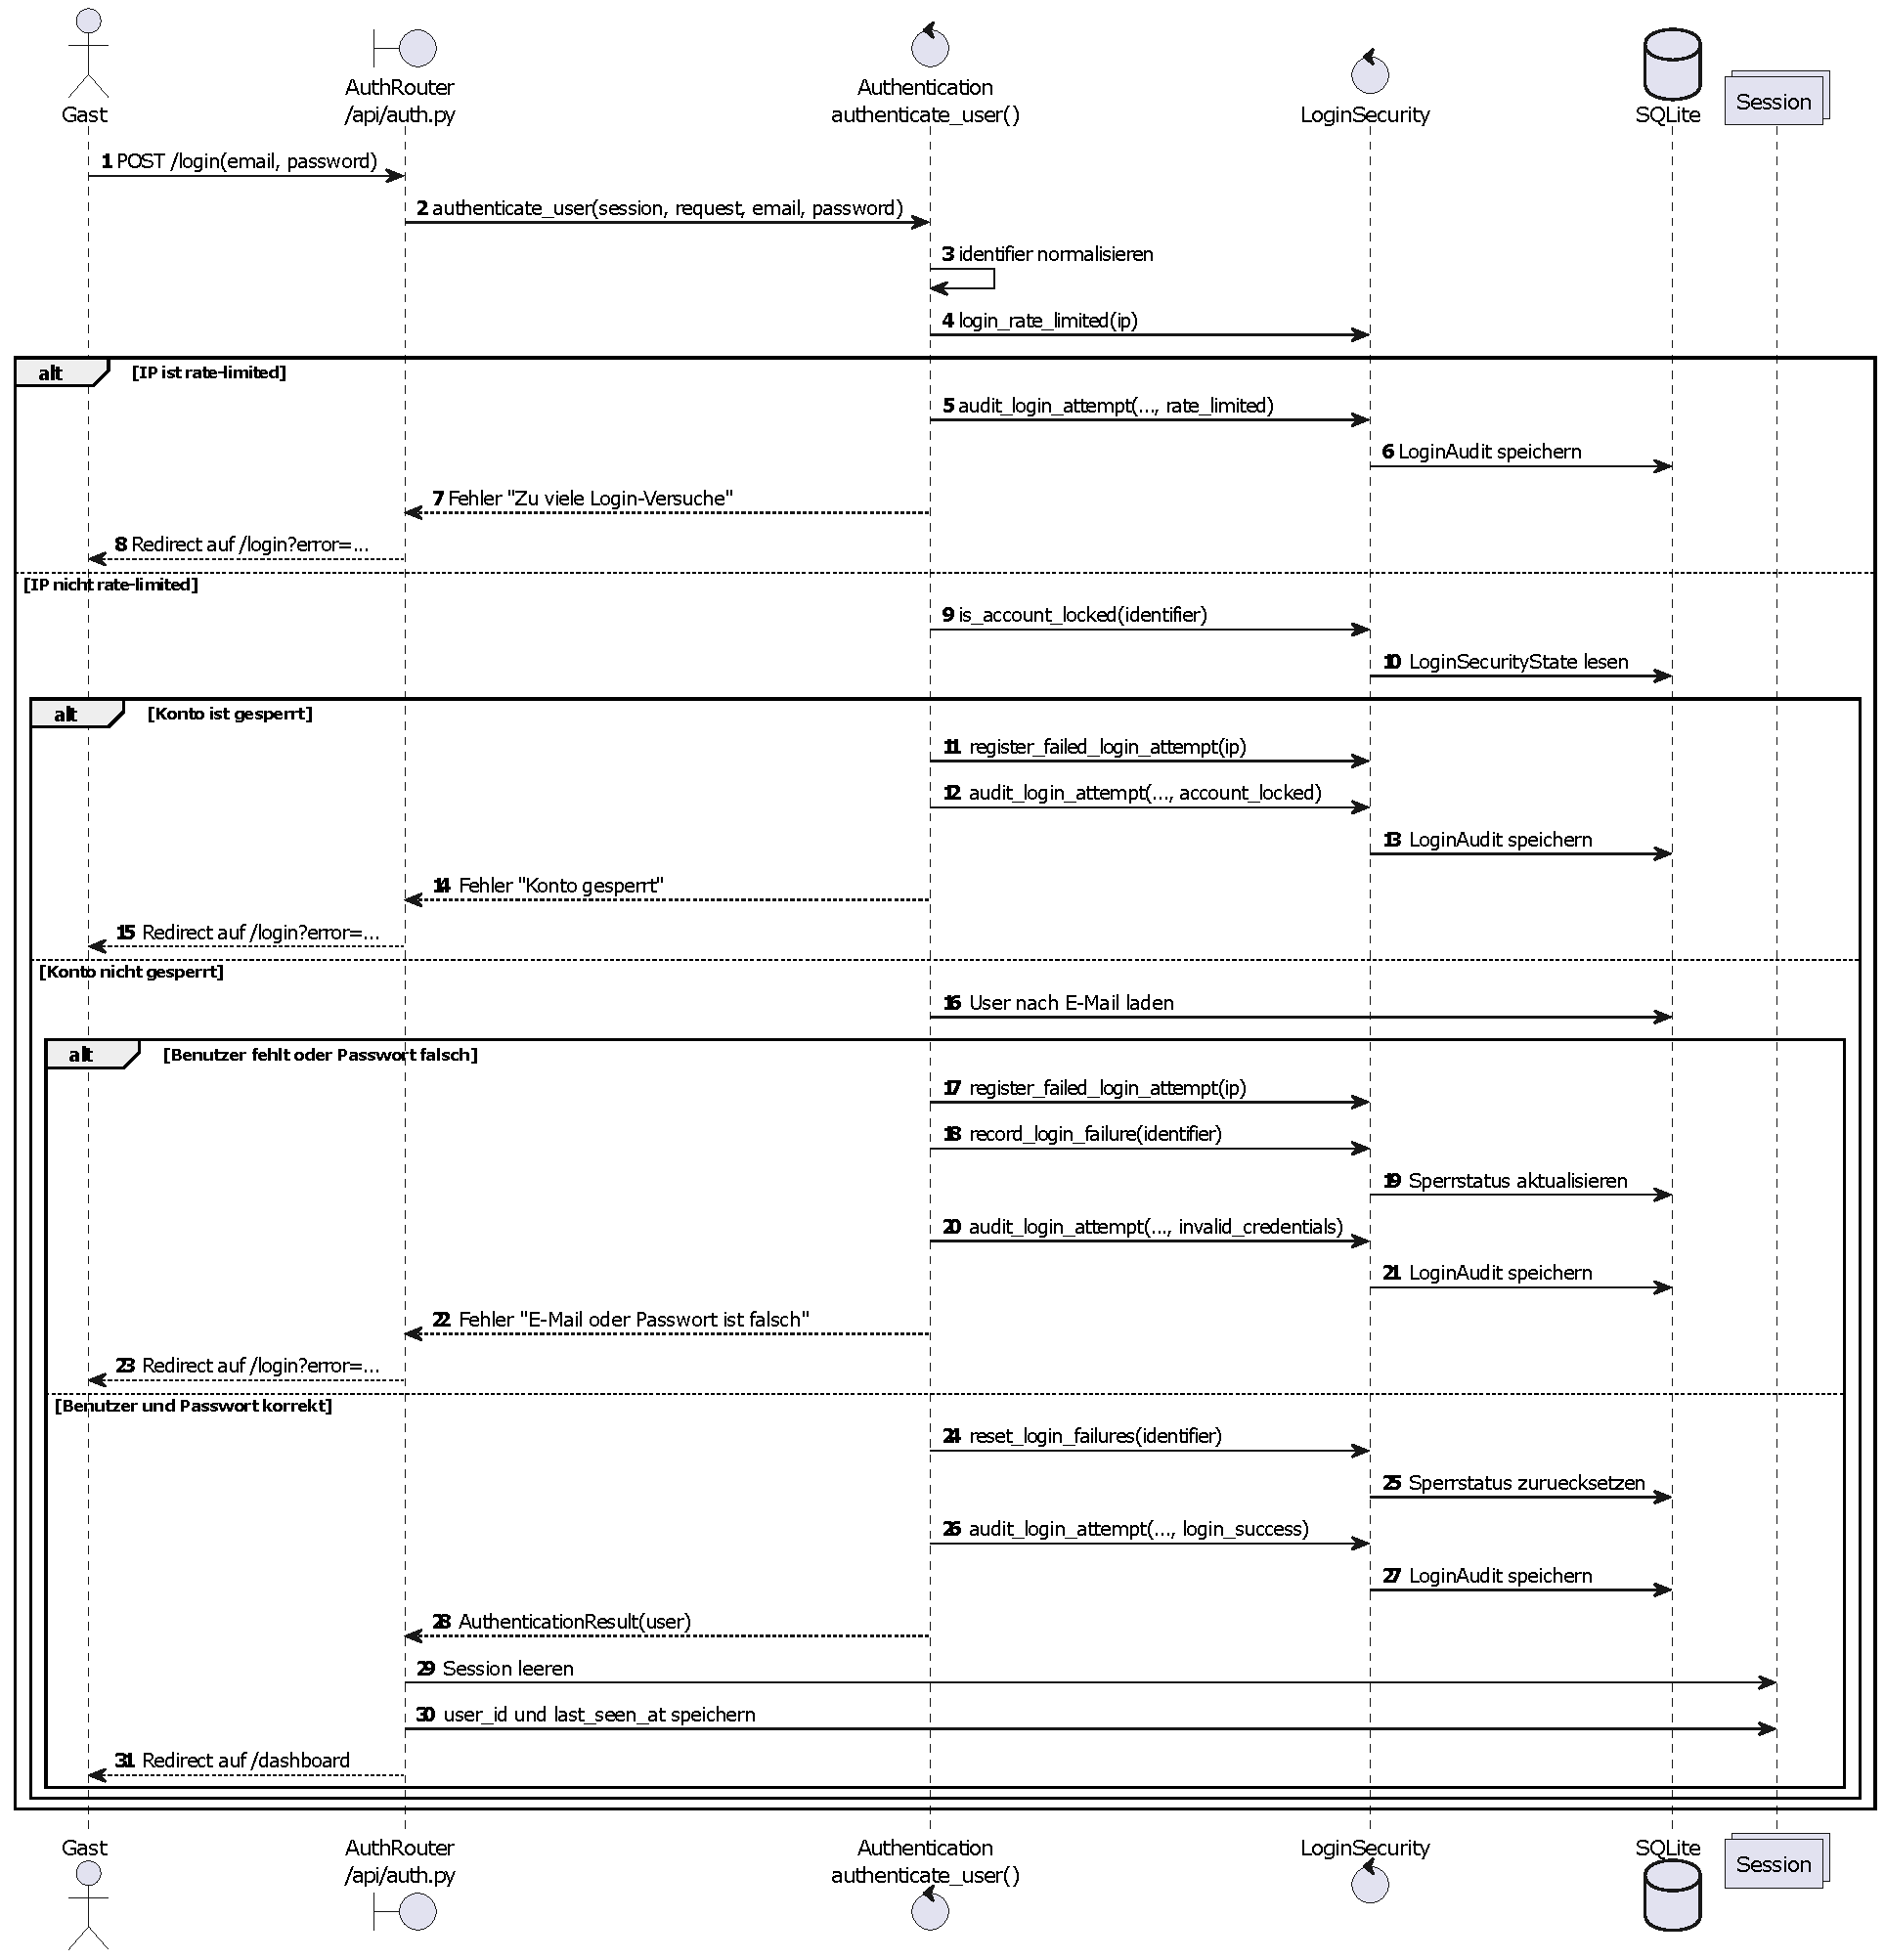
\includegraphics[width=0.95\textwidth]{PlantUML/Sequenzdiagramm_Login.pdf}
\caption{Sequenzdiagramm Login}
\end{figure}
\clearpage

\subsection{Kundenhinweis}
\label{app:Kundenhinweis}
Die Anwendung ist für die tägliche Pflege von Organisationen, Benutzern,
Mail-Adressen und IP-Adressen vorgesehen. Vor dem Löschen eines Datensatzes
soll geprüft werden, ob der Eintrag noch für nachgelagerte Prozesse benötigt
wird. Fachliche Änderungen sind über das Audit-Log nachvollziehbar.
\clearpage

\subsection{Quelltextauszug Berechtigungslogik}
\label{app:CodeAuthentifizierung}
\lstinputlisting[language=Python, caption={Berechtigungslogik für organisationsbezogene Zugriffe}]{PROJEKT/app/services/permissions.py}
\clearpage

\subsection{Testauszug}
\label{app:Testauszug}
\lstinputlisting[language=Python, caption={Beispielhafte API-Tests für die Benutzerverwaltung}]{PROJEKT/tests/web/api/test_users.py}
